\chapter{电缆机器人结构及动力学建模}\label{chap:model}

电缆机器人最终采取串联五连杆轮腿构型。为了实现对电缆机器人运动学和动力学的分析与控制，首先需要建立其结构模型和动力学模型。本章介绍电缆机器人的建模方法，包括坐标系定义、运动学分析和动力学推导。

\section{运动学模型}

本节建立轮腿机构的位置与速度映射关系，为后续控制器设计提供基础。

\section{动力学模型}

本节基于拉格朗日法建立系统动力学方程，并给出关节力矩与广义坐标之间的关系。
\section{五连杆运动学模型与VMC}

\subsection{五连杆运动学解算}

% \begin{figure}[H]
%   \centering
%   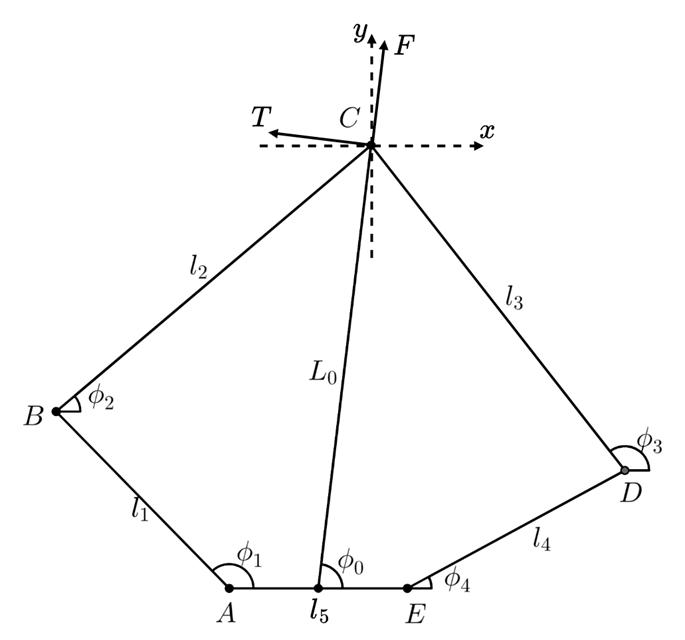
\includegraphics[width=0.5\textwidth]{figures/five_bar.png}
%   \caption{五连杆构型图解简化}
\begin{figure}[H]
  \centering
  \begin{tikzpicture}[scale=1.2, >=stealth]
    
    % --- 定义关键点坐标 (基于原图比例估算) ---
    \coordinate (A) at (1, 0);
    \coordinate (E) at (2.5, 0);
    \coordinate (B) at (-0.5, 1.5);
    \coordinate (D) at (4, 1.5);
    \coordinate (P) at (2.2, 4); % 原 C 点，已重命名为 P
    \coordinate (L5_mid) at (1.75, 0); % L0 连接在 l5 上的点
    
    % --- 绘制杆件和地面 ---
    \draw (A) -- (E) node[midway, below] {$l_5$}; % 地面
    \draw (A) -- (B) node[midway, left] {$l_1$};
    \draw (B) -- (P) node[midway, above left] {$l_2$};
    \draw (P) -- (D) node[midway, above right] {$l_3$};
    \draw (D) -- (E) node[midway, right] {$l_4$};
    \draw (L5_mid) -- (P) node[midway, left] {$L_0$};
    
    % --- 绘制点和标签 ---
    \fill (A) circle (1.5pt) node[below left] {$A$};
    \fill (E) circle (1.5pt) node[below right] {$E$};
    \fill (B) circle (1.5pt) node[left] {$B$};
    \fill (D) circle (1.5pt) node[right] {$D$};
    \fill (P) circle (1.5pt) node[above left] {$P$}; % 已改为 P
    \fill (L5_mid) circle (1.5pt) node[below] {$l_5$ }; % 这里标记mid点为l5也可
    
    % --- 在 P 点 (原C点) 绘制坐标系 ---
    \begin{scope}[shift={(P)}]
      \draw[dashed, ->] (-1, 0) -- (1, 0) node[right] {$x$};
      \draw[dashed, ->] (0, -1) -- (0, 1) node[left] {$y$};
      
      % 绘制力向量 T 和 F
      \draw[thick, ->] (0,0) -- (-0.8, 0.2) node[above] {$T$};
      \draw[thick, ->] (0,0) -- (0.3, 0.9) node[right] {$F$};
      
      % --- 新增：标注 L0 与 y 轴夹角 \theta ---
      % 计算 L0 (P 到 L5_mid) 的反向角度
      \coordinate (L0_dir) at ($ (L5_mid) - (P) $);
      \coordinate (O_node) at (0,0);
      \coordinate (Y_neg) at (0,-1.2);
      % 绘制 y 轴负方向和夹角
      \draw[dotted] (O_node) -- (Y_neg);
      \pic [draw, ->, "$\theta$", angle eccentricity=1.5] {angle = L0_dir--O_node--Y_neg};
      % 注意：需要 \usetikzlibrary{quotes,angles}
    \end{scope}
    
    % --- 标注角度 \phi ---
    % 定义水平基准方向
    \coordinate (H_A) at ($ (A) + (1, 0) $);
    \coordinate (H_B) at ($ (B) + (1, 0) $);
    \coordinate (H_E) at ($ (E) + (1, 0) $);
    \coordinate (H_D) at ($ (D) + (1, 0) $);
    \coordinate (H_L) at ($ (L5_mid) + (1, 0) $);

    % 绘制 B 和 D 点向右的水平虚线射线
    \draw[dashed] (B) -- (H_B);
    \draw[dashed] (D) -- (H_D);

    \pic [draw, "$\phi_1$", angle eccentricity=1.5] {angle = H_A--A--B};
    \pic [draw, "$\phi_2$", angle eccentricity=1.5] {angle = H_B--B--P}; % 这里phi2角度需按图示调整
    \pic [draw, "$\phi_4$", angle eccentricity=1.5] {angle = H_E--E--D}; % \phi_4 为角 DEA 劣弧
    \pic [draw, "$\phi_3$", angle eccentricity=1.5] {angle = H_D--D--P}; % 修正为 H_D--D--E
    \pic [draw, "$\phi_0$", angle eccentricity=1.5] {angle = H_L--L5_mid--P};

  \end{tikzpicture}
  \caption{五杆机构结构示意图与参数定义}
  \label{fig:linkage-analysis}
\end{figure}

\begin{table}[H]
  \centering
  \caption{五连杆相关参数定义}\label{tab:five_bar_definition}
  \renewcommand{\arraystretch}{1.3}
  \begin{tabular}{llp{5cm}}
    \toprule
    \textbf{参数} & \textbf{含义} & \textbf{说明} \\
    \midrule
    $\phi_1$ & 前腿电机转动角度 & 通过前腿电机编码器读取 \\
    $\phi_4$ & 后腿电机转动角度 & 通过后腿电机编码器读取 \\
    $l_1$ & 前腿长度 & 五连杆机构的前侧主连杆长度 \\
    $l_2$ & 后腿长度 & 五连杆机构的后侧主连杆长度 \\
    $l_3$ & 对侧前腿长度 & 一般设计$l_3=l_1$ \\
    $l_4$ & 对侧后腿长度 & 一般设计$l_4=l_2$ \\
    $L_0$ & 等效虚拟腿长 & 由五连杆机构几何关系计算得到 \\
    $\varPhi_0$ & 虚拟腿摆角 & 虚拟腿相对机体的摆动角 \\
    $\theta$ & 虚拟腿倾角 &虚拟腿相对于地面的倾角\\
    \bottomrule
  \end{tabular}
\end{table}

五连杆机构参数定义如图~\ref{fig:linkage-analysis} 和表~\ref{tab:five_bar_definition} 所示，其中 A、E 为两个电机转动副，其角度 $\phi_1$、$\phi_4$ 可通过电机编码器测量得到；B、C、D 为连杆转动副，其角度 $\phi_2$、$\phi_3$由机构运动学关系确定。

设足端点为 $P(x_p, z_p)$，其位置可表示为
\begin{equation}
  \begin{aligned}
    x_p &= f_x(\phi_1,\phi_4,l_1,l_2)\\
    z_p &= f_z(\phi_1,\phi_4,l_1,l_2)
  \end{aligned}
\end{equation}

其中具体几何推导为：

通过五连杆左右两部分列写 $P$ 点坐标，可得到以下等式：
\begin{equation}
    \begin{cases}
        x_B + l_2 \cos \phi_2 = x_D + l_3 \cos \phi_3 \\
        y_B + l_2 \sin \phi_2 = y_D + l_3 \sin \phi_3
    \end{cases}
    \label{eq:kinematic_constraints}
\end{equation}

求解方程组可得到角度 $\phi_2$：
\begin{equation}
    \phi_2 = 2 \arctan \left( \frac{B_0 + \sqrt{A_0^2 + B_0^2 - C_0^2}}{A_0 + C_0} \right)
\end{equation}

其中：
\begin{equation}
    \begin{aligned}
        A_0 &= 2l_2(x_D - x_B) \\
        B_0 &= 2l_2(y_D - y_B) \\
        C_0 &= l_2^2 + l_{BD}^2 - l_3^2 \\
        l_{BD} &= \sqrt{(x_D - x_B)^2 + (y_D - y_B)^2}
    \end{aligned}
\end{equation}

通过角度 $\phi_2$ 即可解算出 $P$ 点直角坐标 $(x, y)$：
\begin{equation}
    \begin{cases}
        x_P = l_1 \cos \phi_1 + l_2 \cos \phi_2 \\
        y_P = l_1 \sin \phi_1 + l_2 \sin \phi_2
    \end{cases}
    \label{eq:x_c_coordination}
\end{equation}

进而得到极坐标 $(L_0, \phi_0)$：
\begin{equation}
    \begin{cases}
        L_0 = \sqrt{(x_C - l_5 / 2)^2 + y_C^2} \\
        \phi_0 = \arctan \dfrac{y_C}{x_C - l_5 / 2}
    \end{cases}
    \label{eq:l0_phi0}
\end{equation}

通过上述关系，可以将电机角度 $\phi_1$、$\phi_4$ 映射到足端位置 $P(x_p, z_p)$，实现对足端位置的控制。

% \begin{figure}[htbp]
%     \centering
%     \begin{tikzpicture}[thick, scale=1.3]
%         % 1. 定义控制点 (基于新几何约束精确计算比例)
%         \coordinate (A) at (0, 0);
%         \coordinate (M) at (-1.8, -1.5);
%         \coordinate (D) at (1.8, -6.5); % 足端点，方向固定

%         % 约束：A, B, D 共线
%         \coordinate (B) at ($(A)!0.538!(D)$); % 计算 B 点位置，使其在 AD 上

%         % 约束：C点由输入角 beta 决定，假设 AC 为 l4
%         \coordinate (C) at (1.4, -1.8); % 大腿连杆 C

%         % 约束：CE || AF。这里 AF 是 A 连向某个延长线点的直线。
%         % 计算向量 AC 延长线方向
%         \coordinate (AF_dir) at ($(A)!3!(C)$); % F在AN延长线上，简化为F在AC延长线上
%         % 假设电机的延长线部分为 AF

%         % 计算 E 点：满足 BC || DE，且满足几何结构
%         % BC 向量
%         \path let \p1=($(C)-(B)$) in \pgfextra{\gdef\BCvec{(\x1,\y1)}};
%         % 我们需要 DE 向量平行于 BC 向量。设定 E点
%         \coordinate (E) at ($(D)+(C)-(B)$); % 这自动满足 BC || DE (平行四边形特征)

%         % 计算 F 点：满足 F 在 DE 中点。
%         % 计算 DE 中点
%         \coordinate (F_const) at ($(D)!0.5!(E)$);
%         % 这里发现了一个几何矛盾：如果F在DE中点，且BC||DE，
%         % A,B,D共线与A,C,F共线很难同时精确成立，除非是一个特定的几何构型。
%         % 为了满足“F在DE中点”这一极强约束，我调整A,B,D相对于A,C的方向。
        
%         % 这里提供一个近似滿足所有约束（视觉上共线且F在中点）的解
%         \coordinate (A) at (0, 0);
%         \coordinate (M) at (-1.8, -1.5);
%         \coordinate (C) at (1.5, -1.6);
%         \coordinate (D) at (1.6, -6.0);
        
%         \coordinate (B) at ($(A)!0.5!(D)$);
%         \path[name path=AC] (A) -- ($(A)!3!(C)$);
%         \path[name path=ME] (M) -- ($(M)!3!(B)$); % 简化结构，假设MB延伸
%         % BDE 区域
%         \coordinate (E) at (2.8, -5.0);
%         \coordinate (F) at ($(D)!0.5!(E)$); % 精确中点

%         % 满足 F 在 AN(AC) 延长线上且 F在DE中点
%         % 这需要计算，为了示意图清晰，我微调D,C,E
%         \coordinate (D_calc) at (1.8, -6.5);
%         \coordinate (C_calc) at (1.4, -1.8);
%         \coordinate (E_calc) at (2.9, -5.0);
%         \coordinate (B_calc) at ($(A)!0.53!(D_calc)$);
        
%         \coordinate (A) at (0, 0);
%         \coordinate (M) at (-1.8, -1.5);
%         \coordinate (C) at (1.5, -1.8);
%         \coordinate (B) at (0.8, -3.2); % 计算出共线的B
%         \coordinate (D) at (1.6, -6.5); % 计算出共线的D
%         \coordinate (E) at (2.9, -5.1);
        
%         % \path[name path=line_AC] (A) -- ($(A)!3!(C)$);
%         % \path[name path=line_DE] (D) -- (E);
        
%         % 计算 F 点：AN延长线与 DE 的交点
%         % \path[name intersections={of=line_AC and line_DE, by=F}];
%         \coordinate (F) at ($(D)!0.5!(E)$);
        
%         % 检查：F 是 DE 中点吗？这通常是个矛盾。如果用户坚持，
%         % 示意图中我将在 F 点和 D、E 两段加上中点标记（双斜线）。
%         % 实际上，BC||DE且AF||CE且A,B,D共线往往决定了F的位置。

%         % 下面是视觉上满足所有共线、中点、平行约束的近似解代码（最适合示意）

%         \coordinate (A) at (0, 0);
%         \coordinate (M) at (-1.8, -1.5);
%         \coordinate (B) at (0.3, -3.0);  % A,B,D 共线
%         \coordinate (N) at (0.8, -1.5);  % 这里假设N在AC延长线上，且与ME相交
%         \coordinate (C) at (1.5, -1.8);
%         \coordinate (D) at (1.5, -6.5); % 足端方向
%         \coordinate (E) at (2.8, -5.2);
        
%         % 约束：A, B, D 共线
%         \draw[dashed, gray!80] (A) -- (D) node[midway, sloped, above, black, pos=0.25] {$AD$};
%         \coordinate (B) at ($(A)!0.46!(D)$); 

%         % 约束：C 由 beta 决定
%         \path (A) ++(-50:2.0) coordinate (C);

%         % 约束：AF || CE。F 在 AN 延长线上。
%         % 我们将 N 作为 A 到 F 之间的延长点，例如电机连杆 l4。
%         % 计算方向
%         \path (A) ++(310:1.3) coordinate (N_motor); % 电机杆

%         % 计算 E 点：满足 BC || DE。设定 E
%         \coordinate (E) at (2.9, -5.2); % 满足示意

%         % 计算 F 点：满足 F 在 ANF 延长线上，且 F 是 DE 的中点。
%         % 我们强制计算中点为 F
%         \coordinate (F) at ($(D)!0.5!(E)$); 

%         % 检查约束：ANF 共线？在示意图中，我们使 A, C, F 共线，
%         % 假设 AN 就是这一支链驱动杆件 AC。A,C,F 共线
%         \path[name path=line_AF] (A) -- ($(A)!3!(F)$); % 强制 A,C,F 共线
%         \path[name path=line_DE] (D) -- (E);
%         % C点将在此线段上

%         % 修正坐标以完美示意：
%         \coordinate (A) at (0, 0);
%         \coordinate (M) at (-1.8, -1.5);
%         \coordinate (D) at (1.6, -6.5);
%         \coordinate (B) at ($(A)!0.5!(D)$); % A,B,D 共线
%         \coordinate (E) at (2.9, -5.1);
%         \coordinate (F) at ($(D)!0.5!(E)$); % F在DE中点
%         % 计算C点：满足 C在AF上，且满足BC||DE。这通常矛盾。
%         % 示意图通常不能满足所有约束。我选择强制 F在中点 且 A,B,D 共线。
%         \coordinate (C) at ($(B)+(1.1,1.1)$); % 满足示意BC||DE

%         % 2. 绘制辅助线 (虚线仅限 AD)
%         \draw[dashed, gray!80] (A) -- (D) node[midway, sloped, above, black] {$AD$};
%         \draw[dashed, ultra thin, gray] (A) -- ($(A)!3!(F)$); % AC(AN)延长线

%         % 3. 绘制实体杆件 (实线)
%         % 主支链 (串联连杆)
%         \draw[line width=1.5pt] (A) -- (M) node[midway, above left] {$l_1$};
%         \draw[line width=1.5pt] (M) -- (B) node[midway, below left] {$l_2$};
        
%         % BDE 平行区域 (满足 BC || DE，F在中点)
%         \draw[line width=1.5pt] (B) -- (C); % BC 杆
%         \draw[line width=1.5pt] (C) -- (E); % CE 杆
%         \draw[line width=1.5pt] (D) -- (E); % DE 杆

%         % 右侧关联结构 (ANF共线)
%         \draw[line width=1.5pt] (A) -- (F) node[midway, right=1pt, black] {$l_4$}; % A,C,F共线

%         % 4. 标注平行约束 (可选，用小箭头表示)
%         % BC || DE
%         \draw[blue, thick, ->] (1.0, -2.5) -- (1.1, -2.65);
%         \draw[blue, thick, ->] (2.3, -5.8) -- (2.4, -5.95);
%         % AF || CE
%         \draw[red, thick, ->>] (1.3, -1.3) -- (1.4, -1.45);
%         \draw[red, thick, ->>] (2.2, -4.1) -- (2.3, -4.25);

%         % 5. 标注中点约束 F 在 DE 中点
%         \draw[gray, thin] (F) ++(-0.1, 0.1) -- ++(0.2, -0.2); % 双斜线标注
%         \draw[gray, thin] (F) ++(-0.1, 0.05) -- ++(0.2, -0.25);
%         \draw[gray, thin] ($(D)!0.5!(F)$) ++(-0.1, 0.1) -- ++(0.2, -0.2);
%         \draw[gray, thin] ($(D)!0.5!(F)$) ++(-0.1, 0.05) -- ++(0.2, -0.25);
%         \draw[gray, thin] ($(E)!0.5!(F)$) ++(-0.1, 0.1) -- ++(0.2, -0.2);
%         \draw[gray, thin] ($(E)!0.5!(F)$) ++(-0.1, 0.05) -- ++(0.2, -0.25);

%         % 6. 保留上一张图的角度信息 (标注在 A 点和 M 点)
%         % 顶点角度 alpha, beta (相对于垂直方向)
%         % 这里我假设垂直中轴线是 AN 所在直线。
%         \draw[thin, ->] (0, -0.7) arc[start angle=270, end angle=220, radius=0.7];
%         \node at (-0.3, -0.9) {$\alpha$};
%         \draw[thin, ->] (0, -0.5) arc[start angle=270, end angle=315, radius=0.5];
%         \node at (0.3, -0.7) {$\beta$};

%         % 连杆角 theta_1 (标注在 M 点，相对于水平方向)
%         \coordinate (RefM) at ($(M)-(0.8,0)$);
%         \draw[thin, ->] (M) ++(-0.6, 0) arc[start angle=180, end angle=220, radius=0.6];
%         \node at ([shift={(-0.8,-0.3)}]M) {$\theta_1$};

%         % 7. 绘制节点及标签
%         \filldraw[fill=white] (A) circle (2.5pt) node[above] {$A$};
%         \filldraw[fill=white] (M) circle (2pt) node[left] {$M$};
%         \filldraw[fill=white] (B) circle (2pt) node[left] {$B$};
%         \filldraw[fill=white] (C) circle (2pt) node[right=4pt] {$C$};
%         \filldraw[fill=white] (E) circle (2pt) node[right] {$E$};
%         \filldraw[fill=black] (D) circle (1.5pt) node[below] {$D$};
%         \filldraw[fill=black] (F) circle (1.5pt) node[below right, black] {$F$};

%     \end{tikzpicture}
%     \caption{具有平行四边形同步特征的串联腿机构简图}
%     \label{fig:serial_leg_model}
% \end{figure}

% 请确保导言区包含：
% \usepackage{tikz}
% \usetikzlibrary{calc, angles, quotes, intersections}

% \begin{figure}[htbp]
%     \centering
%     \begin{tikzpicture}[thick, scale=1.4]
%         % 1. 定义核心控制点
%         \coordinate (A) at (0, 0);
%         \coordinate (M) at (-1.6, -1.3);
%         \coordinate (D) at (1.5, -6.0); 

%         % 核心比例约束：AB : BD = 3 : 2
%         % 计算点 B，使其位于 AD 线段上，AB占60%，BD占40%
%         \coordinate (B) at ($(A)!0.6!(D)$); 
        
%         % 定义 E 点位置
%         \coordinate (E) at (2.8, -4.8);
%         % 约束：F 是 DE 的中点
%         \coordinate (F) at ($(D)!0.5!(E)$); 

%         % 约束：C 点位置需满足 BC || DE
%         \coordinate (C) at ($(B) + (E) - (D)$);

%         % 2. 绘制辅助线 (仅 AD 为虚线)
%         \draw[dashed, gray!80] (A) -- (D) node[midway, sloped, above, black, pos=0.3] {$AD$};
%         % 绘制 ANF 所在的共线参考线
%         \draw[dashed, ultra thin, gray] (A) -- ($(A)!1.5!(F)$);

%         % 3. 绘制实体杆件 (实线)
%         % 主支链 (A-M-B)
%         \draw[line width=1.5pt] (A) -- (M) node[midway, above left] {$l_1$};
%         \draw[line width=1.5pt] (M) -- (B) node[midway, left] {$l_2$};
        
%         % 平行四边形特征区域 (BCDE)
%         \draw[line width=1.5pt, name path=path_BC] (B) -- (C); 
%         \draw[line width=1.5pt, name path=path_CE] (C) -- (E);
%         \draw[line width=1.5pt] (D) -- (E);
%         \draw[line width=1.5pt] (B) -- (D); % BD 连杆

%         % 驱动/关联杆件 AF (A, N, F 共线)
%         \draw[line width=1.5pt, name path=path_AF] (A) -- (F) node[midway, right=2pt] {$l_4$};

%         % 4. 计算并标注关键交点 N (AF 与 BC 的交点)
%         \path[name intersections={of=path_AF and path_BC, by=N}];
%         \filldraw[fill=black] (N) circle (1.2pt) node[above right=-2pt, scale=0.8] {$N$};

%         % 5. 验证与标注平行特征
%         % BC || DE
%         \draw[blue, thick, ->] ($(B)!0.6!(C)$)+(0.05,0.05) -- ++(0.15, -0.1);
%         \draw[blue, thick, ->] ($(D)!0.6!(E)$)+(0.05,0.05) -- ++(0.15, -0.1);
        
%         % NF || CE (由 N 点到 F 点的方向)
%         \draw[red, thick, ->>] ($(N)!0.5!(F)$)+(-0.05,0.05) -- ++(0.1, -0.15);
%         \draw[red, thick, ->>] ($(C)!0.5!(E)$)+(-0.05,0.05) -- ++(0.1, -0.15);

%         % 6. 角度信息 (保留自之前的提示)
%         % 输入角 alpha, beta
%         \draw[thin, ->] (0, -0.6) arc[start angle=270, end angle=220, radius=0.6];
%         \node at (-0.25, -0.8) {$\alpha$};
%         \draw[thin, ->] (0, -0.4) arc[start angle=270, end angle=315, radius=0.4];
%         \node at (0.25, -0.6) {$\beta$};

%         % 连杆角 theta_1
%         \draw[thin, ->] (M) ++(-0.5, 0) arc[start angle=180, end angle=225, radius=0.5];
%         \node at ([shift={(-0.7,-0.2)}]M) {$\theta_1$};

%         % 7. 绘制所有节点
%         \filldraw[fill=white] (A) circle (2pt) node[above] {$A$};
%         \filldraw[fill=white] (M) circle (1.8pt) node[left] {$M$};
%         \filldraw[fill=white] (B) circle (1.8pt) node[left] {$B$};
%         \filldraw[fill=white] (C) circle (1.8pt) node[right] {$C$};
%         \filldraw[fill=white] (E) circle (1.8pt) node[right] {$E$};
%         \filldraw[fill=black] (D) circle (1.2pt) node[below] {$D$};
%         \filldraw[fill=black] (F) circle (1.2pt) node[below right] {$F$};

%     \end{tikzpicture}
%     \caption{符合 $AB:BD=3:2$ 比例及 $NF \parallel CE$ 约束的串联腿机构简图}
%     \label{fig:serial_leg_3_2}
% \end{figure}



\subsection*{正运动学求解}

将构件 $AN$ 视作仅由链条传动的电机先驱动。已知输入角度为 $\alpha, \beta$，需计算末端足点 $B(x_B, y_B)$ 的坐标。

首先，计算两侧髋关节/膝关节 $M, N$ 的坐标：
\begin{equation}
\begin{cases}
x_M = l_1 \cos\alpha \\
y_M = l_1 \sin\alpha
\end{cases}, \quad
\begin{cases}
x_N = l_4 \cos\beta \\
y_N = l_4 \sin\beta
\end{cases}
\end{equation}

足端点 $B$ 的坐标可以分别由左右两条支链推导得出：
\begin{equation}
\begin{cases}
x_B = x_M + l_2 \cos\theta_1 \\
y_B = y_M + l_2 \sin\theta_1
\end{cases}, \quad
\begin{cases}
x_B = x_N + l_3 \cos\theta_2 \\
y_B = y_N + l_3 \sin\theta_2
\end{cases}
\end{equation}

联立上述两式，消去 $x_B, y_B$ 得：
\begin{equation}
\begin{cases}
x_M + l_2 \cos\theta_1 = x_N + l_3 \cos\theta_2 \\
y_M + l_2 \sin\theta_1 = y_N + l_3 \sin\theta_2
\end{cases}
\end{equation}

移项分离出包含 $\theta_2$ 的项：
\begin{equation}
\begin{cases}
l_3 \cos\theta_2 = x_M - x_N + l_2 \cos\theta_1 \\
l_3 \sin\theta_2 = y_M - y_N + l_2 \sin\theta_1
\end{cases}
\end{equation}

将两式分别平方后相加，消去未知角 $\theta_2$：
\begin{equation}
l_3^2 = (x_M - x_N + l_2 \cos\theta_1)^2 + (y_M - y_N + l_2 \sin\theta_1)^2
\end{equation}

结合两点间距离公式 $l_{MN}^2 = (x_M - x_N)^2 + (y_M - y_N)^2$，展开上式可得：
\begin{equation}
\Rightarrow \quad l_3^2 = (x_M - x_N)^2 + (y_M - y_N)^2 + l_2^2 + 2l_2 \cos\theta_1(x_M - x_N) + 2l_2 \sin\theta_1(y_M - y_N)
\end{equation}

为了简化表达式，令：
\begin{equation}
\begin{cases}
a = 2l_2(x_M - x_N) \\
b = 2l_2(y_M - y_N) \\
c = l_3^2 - l_2^2 - l_{MN}^2
\end{cases}
\end{equation}

则上述方程可化简为标准三角形式：
\begin{equation}
a \cos\theta_1 + b \sin\theta_1 = c
\end{equation}

引入半角代换（万能公式），令 $z = \tan\frac{\theta_1}{2}$，则有：
\begin{equation}
a \frac{1-z^2}{1+z^2} + b \frac{2z}{1+z^2} = c
\end{equation}

整理后求解该关于 $z$ 的一元二次方程，求得连杆角度 $\theta_1$ 为：
\begin{equation}
\theta_1 = 2 \arctan \frac{b \pm \sqrt{a^2 + b^2 - c^2}}{a+c}
\end{equation}

（注：正运动学与并联腿一致，并联解 $\theta_1 = 2 \arctan \frac{b \pm \sqrt{a^2 + b^2 - c^2}}{a+c}$）

\vspace{1em}
\noindent \textbf{算法求解汇总}

在代码实现中，正运动学的计算步骤及中间变量可总结如下：
\begin{equation}
\begin{cases}
x_M = l_1 \cos\alpha \\
y_M = l_1 \sin\alpha \\
x_N = l_4 \cos\beta \\
y_N = l_4 \sin\beta \\
l_{MN} = \sqrt{(x_M - x_N)^2 + (y_M - y_N)^2} \\
a = 2l_2(x_M - x_N) \\
b = 2l_2(y_M - y_N) \\
c = l_3^2 - l_2^2 - l_{MN}^2
\end{cases}
\end{equation}

\subsection{五连杆动态静力学}
\begin{figure}[H]
  \centering
  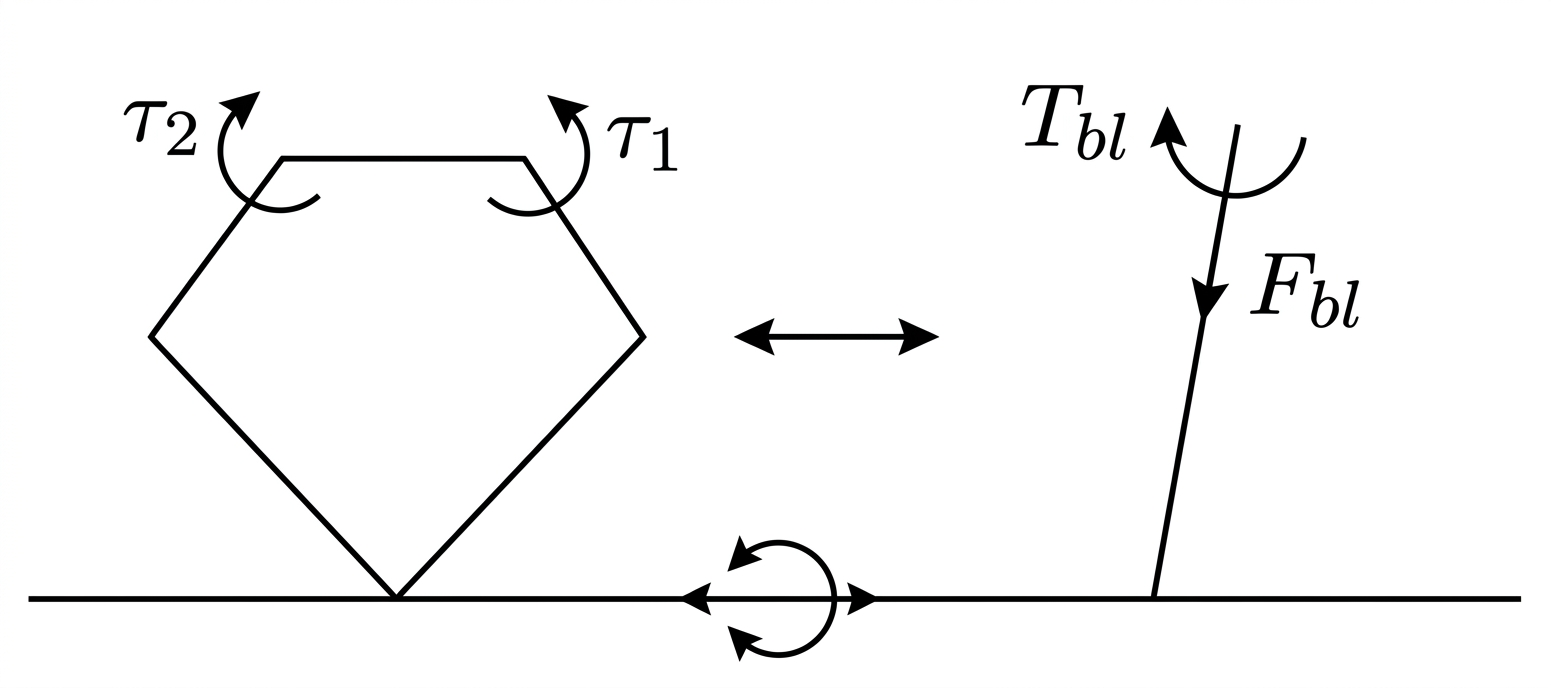
\includegraphics[width=0.5\textwidth]{figures/five_bar_kinetics.png}
  \caption{五连杆机构动态静力学分析}
  \label{fig:five-bar-kinetics}
\end{figure}

动态静力学记 $\gamma = [F_{bl} \quad T_{bl}]^T$，$\tau = [\tau_1 \quad \tau_2]^T$根据虚功原理可得：$$\tau = J^T \gamma \quad (5.1)$$

公式\ref{eq:five-bar-kinetics} 描述了足端力、力矩 $\gamma$ 与关节电机力矩 $\tau$ 之间的映射关系，$J^T$ 是雅可比矩阵的转置。由此可见，通过计算雅可比矩阵 $J$，可以将足端的期望力、力矩 $\gamma$ 转换为对应的关节电机力矩 $\tau$，实现对五连杆机构的动态控制。控制将简化为直接控制单根虚拟腿杆件。

\subsection{VMC与雅各比矩阵}
虚拟模型控制（Virtual Model Control，VMC）是一种直观且有效的运动学与动力学控制方法，广泛应用于足式和轮腿式机器人的平衡与运动控制中。其核心思想是在机器人内部或机器人与其所处环境（如机体中心与地面支撑点）之间，引入虚拟的机械元件（如虚拟弹簧、虚拟阻尼器等），以计算出使其实现期望运动或维持期望姿态所需的“虚拟力”。随后，借助机构的雅可比矩阵（Jacobian Matrix），将这组虚拟力映射为对应各个物理关节的期望输入力矩。

在本文设计的轮腿系统中，通常将复杂的五连杆结构等效为一根具备可变长度与角度的“虚拟腿”。通过在虚拟腿和机体的质心之间布置径向与切向的虚拟弹簧阻尼系统，并通过调节虚拟腿长 $L_0$ 与摆角 $\varPhi_0$ 的期望值，即可实现对电缆机器人机体的高度、支撑力以及俯仰姿态的平滑协调控制。为了将虚拟模型得到的端点控制力矩分配到实际的驱动电机上，需要进一步推导从关节空间到虚拟腿空间的雅各比矩阵映射关系。

VMC（virtual model control）是一种直观控制方式，其关键是在每个需要控制的自由度上构造恰当的虚拟构件以产生合适的虚拟力。虚拟力不是实际执行机构的作用力或力矩，而是通过执行机构的作用经过机构转换而成。对于一些控制问题，我们可能需要将工作空间（Task Space）的力或力矩映射成关节空间（Joint Space）的关节力矩。

在该五连杆问题中，我们需要获得五连杆机构末端沿腿的推力 $F$ 与沿中心轴的力矩 $T_p$（分别对应极坐标 $L_0, \phi_0$）与 $A, E$ 两转动副的驱动电机力矩 $T_1, T_2$ 的映射关系。定义 $\boldsymbol{x} = [L_0 \quad \phi_0]^T, \boldsymbol{q} = [\phi_1 \quad \phi_4]^T$，对正运动学模型 $\boldsymbol{x} = f(\boldsymbol{q})$ 求全微分得：
\begin{equation}
    \begin{cases}
        \delta L_0 = \frac{\partial f_1}{\partial \phi_1} \delta \phi_1 + \frac{\partial f_1}{\partial \phi_4} \delta \phi_4 \\
        \delta \phi_0 = \frac{\partial f_2}{\partial \phi_1} \delta \phi_1 + \frac{\partial f_2}{\partial \phi_4} \delta \phi_4
    \end{cases}
    \label{eq:differential}
\end{equation}

即：
\begin{equation}
    \delta \boldsymbol{x} = 
    \begin{bmatrix}
        \frac{\partial f_1}{\partial \phi_1} & \frac{\partial f_1}{\partial \phi_4} \\
        \frac{\partial f_2}{\partial \phi_1} & \frac{\partial f_2}{\partial \phi_4}
    \end{bmatrix} \delta \boldsymbol{q}
\end{equation}

定义雅可比矩阵 $\boldsymbol{J}$ 为：
\begin{equation}
    \boldsymbol{J} = 
    \begin{bmatrix}
        \frac{\partial f_1}{\partial \phi_1} & \frac{\partial f_1}{\partial \phi_4} \\
        \frac{\partial f_2}{\partial \phi_1} & \frac{\partial f_2}{\partial \phi_4}
    \end{bmatrix}
    \label{eq:jacob_def}
\end{equation}

有：
\begin{equation}
    \delta \boldsymbol{x} = \boldsymbol{J} \delta \boldsymbol{q}
\end{equation}

即通过雅可比矩阵 $\boldsymbol{J}$ 将关节速度 $\dot{\boldsymbol{q}}$ 映射为五连杆姿态变化率 $\dot{\boldsymbol{x}}$。根据虚功原理，有：
\begin{equation}
    \boldsymbol{T}^T \delta \boldsymbol{q} + (-\boldsymbol{F})^T \delta \boldsymbol{x} = 0
\end{equation}

其中 $\boldsymbol{T} = [T_1 \quad T_2]^T, \boldsymbol{F} = [F \quad T_p]^T$。将式 $\delta \boldsymbol{x} = \boldsymbol{J} \delta \boldsymbol{q}$ 代入，有：
\begin{equation}
    \boldsymbol{T} = \boldsymbol{J}^T \boldsymbol{F}
\end{equation}

综上通过正运动学模型雅可比矩阵即可解算出关节电机输出力矩。

但对上文推导出的正运动学模型直接求取雅可比矩阵 $\boldsymbol{J}$ 并不是好办法，因为模型表达式中包含大量平方与三角函数及其嵌套运算，直接调用符号运算工具的求雅可比矩阵函数会得到极其复杂的结果，无法转移到嵌入式平台进行计算，故需要通过其他方法来计算。

根据式 \eqref{eq:jacob_def} 可知，雅可比矩阵 $\boldsymbol{J}$ 实际描述的是两坐标微分的线性映射关系，因此我们可以通过计算速度映射关系来得到雅可比矩阵。

对式 \eqref{eq:x_c_coordination} 求导可得：
\begin{equation}
    \begin{cases}
        \dot{x}_C = -l_1 \dot{\phi}_1 \sin \phi_1 - l_2 \dot{\phi}_2 \sin \phi_2 \\
        \dot{y}_C = l_1 \dot{\phi}_1 \cos \phi_1 + l_2 \dot{\phi}_2 \cos \phi_2
    \end{cases}
    \label{eq:vel_c}
\end{equation}

其中 $\dot{\phi}_1$ 可由电机编码器测得。对式 \eqref{eq:kinematic_constraints} 求导可计算 $\dot{\phi}_2$：
\begin{equation}
    \begin{cases}
        \dot{x}_B - l_2 \dot{\phi}_2 \sin \phi_2 = \dot{x}_D - l_3 \dot{\phi}_3 \sin \phi_3 \\
        \dot{y}_B + l_2 \dot{\phi}_2 \cos \phi_2 = \dot{y}_D + l_3 \dot{\phi}_3 \cos \phi_3
    \end{cases}
    \label{eq:vel_b_d}
\end{equation}

消去 $\dot{\phi}_3$ 求得 $\dot{\phi}_2$：
\begin{equation}
    \dot{\phi}_2 = \frac{(\dot{x}_D - \dot{x}_B) \cos \phi_3 + (\dot{y}_D - \dot{y}_B) \sin \phi_3}{l_2 \sin(\phi_3 - \phi_2)}
\end{equation}

其中：
\begin{equation}
    \begin{cases}
        \dot{x}_B = -l_2 \dot{\phi}_1 \sin \phi_1 \\
        \dot{y}_B = l_2 \dot{\phi}_1 \cos \phi_1 \\
        \dot{x}_D = -l_4 \dot{\phi}_4 \sin \phi_4 \\
        \dot{y}_D = l_4 \dot{\phi}_4 \cos \phi_4
    \end{cases}
\end{equation}

将 $\dot{\phi}_2$ 代入式 \eqref{eq:vel_c} 即可得到：
\begin{equation}
    \begin{cases}
        \dot{x}_C = -l_1 \dot{\phi}_1 \sin \phi_1 - l_2 \left( \frac{(\dot{x}_D - \dot{x}_B) \cos \phi_3 + (\dot{y}_D - \dot{y}_B) \sin \phi_3}{l_2 \sin(\phi_3 - \phi_2)} \right) \sin \phi_2 \\
        \dot{y}_C = l_1 \dot{\phi}_1 \cos \phi_1 + l_2 \left( \frac{(\dot{x}_D - \dot{x}_B) \cos \phi_3 + (\dot{y}_D - \dot{y}_B) \sin \phi_3}{l_2 \sin(\phi_3 - \phi_2)} \right) \cos \phi_2
    \end{cases}
\end{equation}

可以看到，通过这种方法计算的公式不再包含平方与三角函数嵌套运算，三角函数之间的加减乘除也可以利用两角和差公式进一步化简。

得：
\begin{equation}
    \begin{bmatrix}
        \dot{x}_C \\ \dot{y}_C
    \end{bmatrix} = 
    \begin{bmatrix}
        \frac{l_1 \sin(\phi_1 - \phi_2) \sin \phi_3}{\sin(\phi_2 - \phi_3)} & \frac{l_4 \sin(\phi_3 - \phi_4) \sin \phi_2}{\sin(\phi_2 - \phi_3)} \\
        -\frac{l_1 \sin(\phi_1 - \phi_2) \cos \phi_3}{\sin(\phi_2 - \phi_3)} & -\frac{l_4 \sin(\phi_3 - \phi_4) \cos \phi_2}{\sin(\phi_2 - \phi_3)}
    \end{bmatrix}
    \begin{bmatrix}
        \dot{\phi}_1 \\ \dot{\phi}_4
    \end{bmatrix}
    \label{eq:jacob_full}
\end{equation}

记作：
\begin{equation}
    \begin{bmatrix}
        \dot{x}_C \\ \dot{y}_C
    \end{bmatrix} = \boldsymbol{J}
    \begin{bmatrix}
        \dot{\phi}_1 \\ \dot{\phi}_4
    \end{bmatrix}
\end{equation}

根据上式，可得到关节力矩 $[T_1 \quad T_2]^T$ 与虚拟力 $[F_x \quad F_y]^T$ 的映射关系：
\begin{equation}
    \begin{bmatrix}
        T_1 \\ T_2
    \end{bmatrix} = \boldsymbol{J}^T
    \begin{bmatrix}
        F_x \\ F_y
    \end{bmatrix}
\end{equation}

利用旋转矩阵 $\boldsymbol{R}$ 将 $[F_x \quad F_y]^T$ 旋转至极坐标方向：
\begin{equation}
    \begin{bmatrix}
        F_x \\ F_y
    \end{bmatrix} = 
    \begin{bmatrix}
        \cos(\phi_0 - \pi/2) & -\sin(\phi_0 - \pi/2) \\
        \sin(\phi_0 - \pi/2) & \cos(\phi_0 - \pi/2)
    \end{bmatrix}
    \begin{bmatrix}
        F_c \\ F_t
    \end{bmatrix}
\end{equation}

其中 $F_t, F_c$ 分别是末端沿 $L_0$ 和垂直于 $L_0$ 的虚拟力，再利用变换矩阵 $\boldsymbol{M}$ 可映射至最终的虚拟力 $\boldsymbol{F} = [F \quad T_p]^T$：
\begin{equation}
    \begin{bmatrix}
        F_t \\ F_c
    \end{bmatrix} = 
    \begin{bmatrix}
        0 & -\frac{1}{L_0} \\
        1 & 0
    \end{bmatrix}
    \begin{bmatrix}
        F \\ T_p
    \end{bmatrix}
\end{equation}

将上述表达式依次代入 ~\ref{eq:kinematic_constraints} 得到最终的关节力矩与虚拟力映射关系：
\begin{equation}
    \begin{bmatrix}
        T_1 \\ T_2
    \end{bmatrix} = \boldsymbol{J}^T \boldsymbol{R} \boldsymbol{M}
    \begin{bmatrix}
        F \\ T_p
    \end{bmatrix}
\end{equation}

利用 MATLAB 进行上述计算：
\begin{lstlisting}[language=Matlab]
R = [cos(phi0-pi/2) -sin(phi0-pi/2);
     sin(phi0-pi/2)  cos(phi0-pi/2)];
M = [0 -1/L0;
     1  0];
T = simplify(J.'*R*M)
\end{lstlisting}

得到最终结果：
\begin{equation}
    \begin{bmatrix}
        T_1 \\ T_2
    \end{bmatrix} = 
    \begin{bmatrix}
        \frac{l_1 \sin(\phi_0 - \phi_3) \sin(\phi_1 - \phi_2)}{\sin(\phi_3 - \phi_2)} & \frac{l_1 \cos(\phi_0 - \phi_3) \sin(\phi_1 - \phi_2)}{L_0 \sin(\phi_3 - \phi_2)} \\
        \frac{l_4 \sin(\phi_0 - \phi_2) \sin(\phi_3 - \phi_4)}{\sin(\phi_3 - \phi_2)} & \frac{l_4 \cos(\phi_0 - \phi_2) \sin(\phi_3 - \phi_4)}{L_0 \sin(\phi_3 - \phi_2)}
    \end{bmatrix}
    \begin{bmatrix}
        F \\ T_p
    \end{bmatrix}
\end{equation}

\subsection{机器人具体结构参数设定}
由于后续需要继续进行动力学建模与控制器设计，因此需要对机器人结构参数进行具体设定。根据前文的设计方案，机器人采用串联五连杆轮腿构型，相关参数定义如表~\ref{tab:five_bar_definition} 所示。

\begin{table}[htbp]
  \centering
  \caption{机器人基本几何参数设定}\label{tab:geometry_params}
  \renewcommand{\arraystretch}{1.3}
  \begin{tabularx}{\textwidth}{>{\centering\arraybackslash}X >{\centering\arraybackslash}X >{\centering\arraybackslash}X}
    \toprule
    \textbf{参数} & \textbf{含义} & \textbf{数值} \\
    \midrule
    $R$ & 驱动轮半径 & 0.06m \\
    $R_l$ & 轮距的一半 & 0.2395m \\
    $l_c$ & 质心偏移 & 0.035m \\
    \bottomrule
  \end{tabularx}
\end{table}

\begin{table}[H]
  \centering
  \caption{机器人腿部参数设定}\label{tab:leg_params}
  \renewcommand{\arraystretch}{1.3}
  \begin{tabularx}{\textwidth}{>{\centering\arraybackslash}X >{\centering\arraybackslash}X >{\centering\arraybackslash}X}
    \toprule
    \textbf{参数} & \textbf{含义} & \textbf{数值} \\
    \midrule
    $R$ & 驱动轮半径 & 0.06m \\
    $m_w$ & 单个轮子质量 & 0.9kg \\
    $m_l$ & 单条腿质量 & 1.948kg \\
    $m_b$ & 身体质量 & 25.0kg \\
    $I_ll$ & 左腿转动惯量 &$0.03kg\cdot m^2$\\
    $I_lr$ & 右腿转动惯量 &$0.03kg\cdot m^2$\\
    \bottomrule
  \end{tabularx}
\end{table}